\documentclass{scrartcl}

\usepackage{tikz}
\usetikzlibrary{positioning, shapes, patterns}
\tikzset{
    state/.style = {draw, align=center, minimum width = 2.1cm, rectangle split, rectangle split parts = 3, thick, minimum height = 5cm},
    tip/.style = {thick, ->, >=stealth}
}
\usepackage{wrapfig}

\usepackage{fontspec}
\setmainfont{Linux Libertine O}

\title{OpenPCells}
\subtitle{Technical Documentation and Implementation Notes}
\author{Patrick Kurth}

\usepackage{kantlipsum}

\begin{document}
\maketitle
\section{Technology Mapping}
Mapping from generic cell descriptions to technology-specific data has to perform several steps:
\begin{itemize}
    \item resolve relative metal numbering
    \item split up via stacks
    \item translate via rectangles to via arrays
    \item map all remaining layers \footnote{The via translation already generates technology-specific layers.}
\end{itemize}

Figure \ref{fig:techtranslation} shows the technology translation from generic to specific cells. This example technology has 7 metal layers, therefor "M-2" points
to "M6".
\begin{figure}[htb]
    \centering
    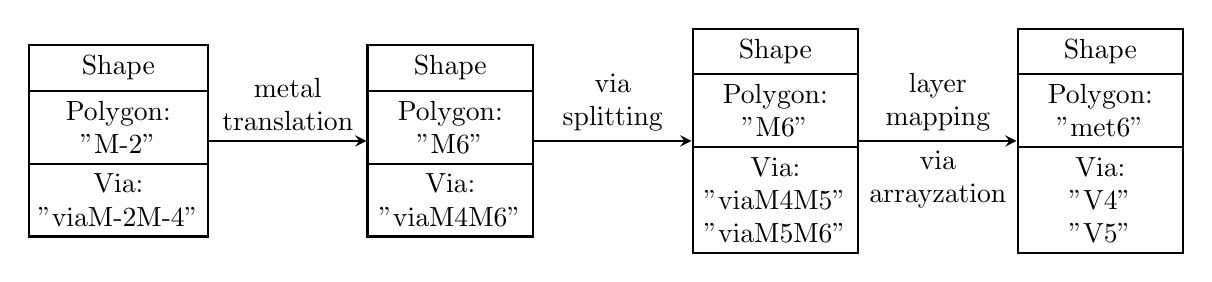
\begin{tikzpicture}
        [
            node distance = 2cm
        ]
        \node[state]                        (initial)  {Shape \nodepart{two} Polygon: \\"M-2" \nodepart{three} Via: \\"viaM-2M-4"};
        \node[state, right = of initial]    (metal)    {Shape \nodepart{two} Polygon: \\"M6"  \nodepart{three} Via: \\"viaM4M6"};
        \node[state, right = of metal]      (via)      {Shape \nodepart{two} Polygon: \\"M6" \nodepart{three} Via: \\"viaM4M5"\\"viaM5M6"};
        \node[state, right = of via]        (layer)    {Shape \nodepart{two} Polygon: \\"met6" \nodepart{three} Via: \\"V4"\\"V5"};
        % arrows
        \draw[tip]  (initial) -- node[above, align = center] {metal\\ translation} (metal);
        \draw[tip]  (metal)   -- node[above, align = center] {via\\ splitting}     (via);
        \draw[tip]  (via)     -- node[above, align = center] {layer\\ mapping} node[below, align = center] {via\\ arrayzation} (layer);
    \end{tikzpicture}
    \caption{Technology translation}
    \label{fig:techtranslation}
\end{figure}

\subsection{Metal Numbering}
For some cells like inductors it is customary to specify things like \emph{last metal} or a metal relative to another. This has to be resolved for further
processing, which is done in this step. Currently, only negative numbers (such as "M-1") are being processed into something like "M8" (depending on the total number
of metals in the technology).
\subsection{Via Splitting}
It is allowed the create via stacks, that is vias with non-adjacent metals. These have to split up into several shapes before via arrayzation.
\subsection{Via Arrayzation}
Via geometries can't be inside generic PCells, since these vary from technology to technology. For this reason, only rectangular areas where vias are to be placed in
a cell are specified. The technology translation then must create the actual via shapes, as shown in figure \ref{fig:viatranslation}.
\begin{wrapfigure}{r}{6cm}
    \centering
    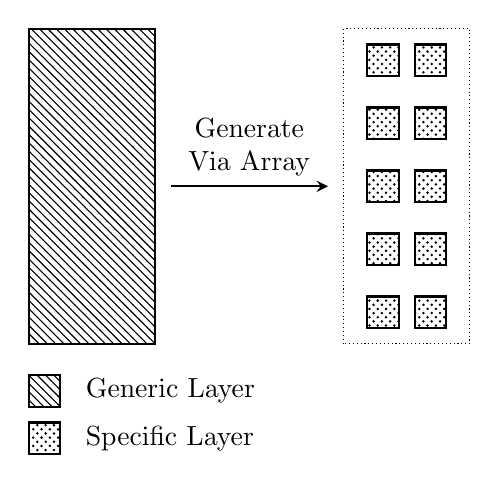
\begin{tikzpicture}[scale = 2]
        \def\viaxsize{0.2}
        \def\viaysize{0.2}
        \draw[thick, pattern = north west lines] (-0.4, -1) rectangle (0.4, 1);
        \draw[densely dotted] (1.6, -1) rectangle (2.4, 1);
        \foreach \x in {-0.15, 0.15}
        {
            \foreach \y in {-0.8, -0.4, 0.0, 0.4, 0.8}
            {
                \draw[thick, pattern = crosshatch dots] 
                    ({2 + \x - 0.5 * \viaxsize}, {\y - 0.5 * \viaysize}) rectangle ({2 + \x + 0.5 * \viaxsize}, {\y + 0.5 * \viaysize});
            }
        }
        \draw[tip] (0.5, 0) -- node[above, align = center] { Generate \\ Via Array } (1.5, 0);
        % legend
        \draw[thick, pattern = north west lines] (-0.4, -1.4) rectangle (-0.2, -1.2);
        \node[anchor = west] at (-0.1, -1.3) {Generic Layer};
        \draw[thick, pattern = crosshatch dots] (-0.4, -1.7) rectangle (-0.2, -1.5);
        \node[anchor = west] at (-0.1, -1.6) {Specific Layer};
    \end{tikzpicture}
    \caption{Example of via arrayzation}
    \label{fig:viatranslation}
\end{wrapfigure}
\subsection{Layer Mapping}

\end{document}

% vim: ft=tex
